We first investigate why weights oscillate in quantization-aware training and how this phenomenon affects neural network training in practice.

\subsection{Quantization-aware training}
\label{sec:qat}
One of the most effective ways to quantize a neural network is by training the network with simulated quantization. During the forward pass, floating-point weights and activation are quantized using the quantization function $q(\cdot)$. It takes input vector $\vec{w}$ and returns quantized output $\vecq{w}$ given by:
\begin{equation}
    \label{eq:quantization_formulation}
    \vecq{w} = q(\vec{w}; s, n, p) = \ct{s} \cdot \clip{\round*{\frac{\vec{w}}{\ct{s}}}}{\ct{n}}{\ct{p}}, 
\end{equation}
where $\round*{\cdot}$ is the \textit{round-to-nearest} operator, $\clip{\cdot}{\alpha}{\beta}$ is a clipping function with lower and upper bounds $\alpha$ and $\beta$, respectively, $\ct{s}$ is a scaling factor, and $\ct{n}$ and $\ct{p}$ the lower and upper quantization thresholds.
In this formulation, the quantized weights $\vecq{w}$ are the ones used during inference, whereas the original floating-point weights $\vec{w}$ only serve as proxies for the optimization and are commonly referred to as \textit{latent weights} or \textit{shadow-weights}.

A fundamental challenge in the QAT formulation is that the rounding function in equation \eqref{eq:quantization_formulation} does not have a meaningful gradient, which makes gradient-based training impossible. One of the most popular techniques for alleviating this issue involves using the straight-through estimator (STE) \cite{bengio2013estimating, hinton2012ste} to approximate the true gradient during training. In practice, this means that we approximate the gradient of the rounding operator as 1 within the quantization limits. We can thus define the gradient of the loss $\tlossb$ with respect to $\vec{w}$ as:
\begin{equation}
    \label{eq:dl_dw_ste}
    \frac{\partial\vec{\tlossb}}{\partial \vec{w}} = \frac{\partial\vec{\tlossb}}{\partial \vecq{w}} \cdot \mathbf{1}_{n \leq \vec{w}/\ct{s} \leq p},
\end{equation}
where $\mathbf{1}$ is the indicator function that is $1$ if $\vec{w}$ falls within the quantization grid, and 0 otherwise, such that there is no gradient outside of the representable quantization region. The STE gradient approximation has been widely adopted in recent literature closing the gap between quantized and full-precision accuracy for a wide range of tasks and networks \citep{Gupta2015, dorefa, krishnamoorthi, tqt, lsq, lsq+, whitepaper}.


\begin{figure*}[ht]
\centering

\includegraphics[width=0.98\textwidth]{figures/toy_example_grad_estimators_100iter.png} \vspace{-.4cm}
\caption{Oscillation  of a single weight in toy-regression problem for various gradient estimator methods: STE (left), EWGS \citep{EWGS} (middle), and DSQ \citep{DSQ} (right).}
\label{fig:oscillation_single_weight}
\end{figure*}

\subsection{Oscillations}
\label{sec:oscillations}
Despite its wide adaptation and enormous success in QAT, the STE  has a counter-intuitive and very interesting side-effect. The STE causes implicit stochasticity during the optimization process due to the latent weights oscillating around the decision boundary between adjacent quantized states. This phenomenon was recently also observed by \citet{diffq}.

To illustrate this, we propose a simple toy regression example that we will refer to frequently throughout this paper.
% We also refer the reader to figure \ref{fig:oscillation_single_weight} for a visual explanation of this example. 
We start with an optimal floating-point weight, $w_*$, as target for our 1D toy regression problem and sample a data vector $\vec{x}$ from a distribution $X$ with bounded variance such that, $\eop{\vec{x}^2}=\sigma^2$, where $0<\sigma^2<\infty$. Then we optimize the least-squares problem
\begin{equation}
    \min_{w}\tlossb(w) = \eopX{\vec{x}\sim X}{\frac{1}{2} \left(\vec{x}w_* - \vec{x}q(w)\right)^2},
    \label{eq:toy_regression_optim}
\end{equation}
where $q(\cdot)$ is the quantizer from equation \eqref{eq:quantization_formulation} and $w$ is the latent weight. We optimize the objective using the STE formulation for the gradients. From figure \ref{fig:oscillation_single_weight} (left), we can see that as the latent weight $w$ approaches the optimal value $w_*$, it starts oscillating around the decision threshold between the quantization levels above $\up{w}$ and below $\down{w}$ the optimal value, as opposed to converging to the region closer to the optimal value $q(w_*)$. 

The weight oscillates around the decision threshold due to the fact that the gradient in equation \eqref{eq:dl_dw_ste} is constant above the threshold, pushing the latent weight down towards $\down{w}$, and constant below the threshold pushing the latent weight up towards $\up{w}$. Please refer to appendix \ref{app:toy_example_gradients} for an analytical expression of this gradient. The induced oscillations happen irrespective of the learning rate. In appendix \ref{app:learning_rates_oscillation} we show that decreasing the learning rate reduces the amplitude of the oscillations but do not affect their frequency.  

The frequency of the oscillation is depends on the distance of the optimal value from its closest quantization level,  $d =|w_* - q(w_*) |$. Let's assume that  $q(w_*)=\up{w}$, then the gradient below the threshold is $k=s/d-1$ times larger than the gradient above, where $s$ is scaling factor or quantization step-size and $s>d$. Interpreting the gradient as the velocity of the latent weight, $w$ needs to travel for $k$ iterations before it crosses the threshold and its velocity/gradient is reversed. In appendix \ref{app:relation_distance_frequency} we show experimentally that the oscillation frequency is indeed directly proportional to closeness of $w_*$ to $q(w_*)$. 

It is interesting to note that this behavior bears similarities to stochastic rounding \citep{Gupta2015}, where the closeness of the latent weight to the quantization level is related to the probability of rounding to that level. However, in STE the source of the stochasticity stems from the discrete nature of the gradients and not from sampling. We note that oscillations are not unique to the vanilla STE, but are present in several variations of the STE proposed in literature, a small subset of which we present in figure \ref{fig:oscillation_single_weight}.

% INCLUDED 
% A side effect of this is that the latent weights themselves are meaningless when the quantizer is removed. A resulting network performs poorly as referenced in \cite{} and as shown in appendix \ref{latent weights don't exisit.}.
 
% Include reference to the 
% The most important information in the updating pattern above is encapsulated not in the latent weight itself, but in the period of its oscillation around the decision boundary. For example, if $w^*$ is closer to $w^+$, the gradient is smaller above the threshold than below. In this case, it follows that the latent weight $w$ spends more time above the decision threshold than below. We see in \ref{somefig} that this is indeed the case, and the period of the oscillation around the decision boundary is directional proportional to the closeness of $w^*$ to $w^+$.

% Stochastic
% similar to what happens in stochastic rounding \cite{}, where the closeness of the latent weight to the grid-point is related to the probability of rounding to that grid-point. However, in the case of the STE, the introduced random process occurs not due to sampling at every iteration, but due to the optimization updates over subsequent iterations. 

\begin{figure}[t]
\centering
\vspace{-.2cm}
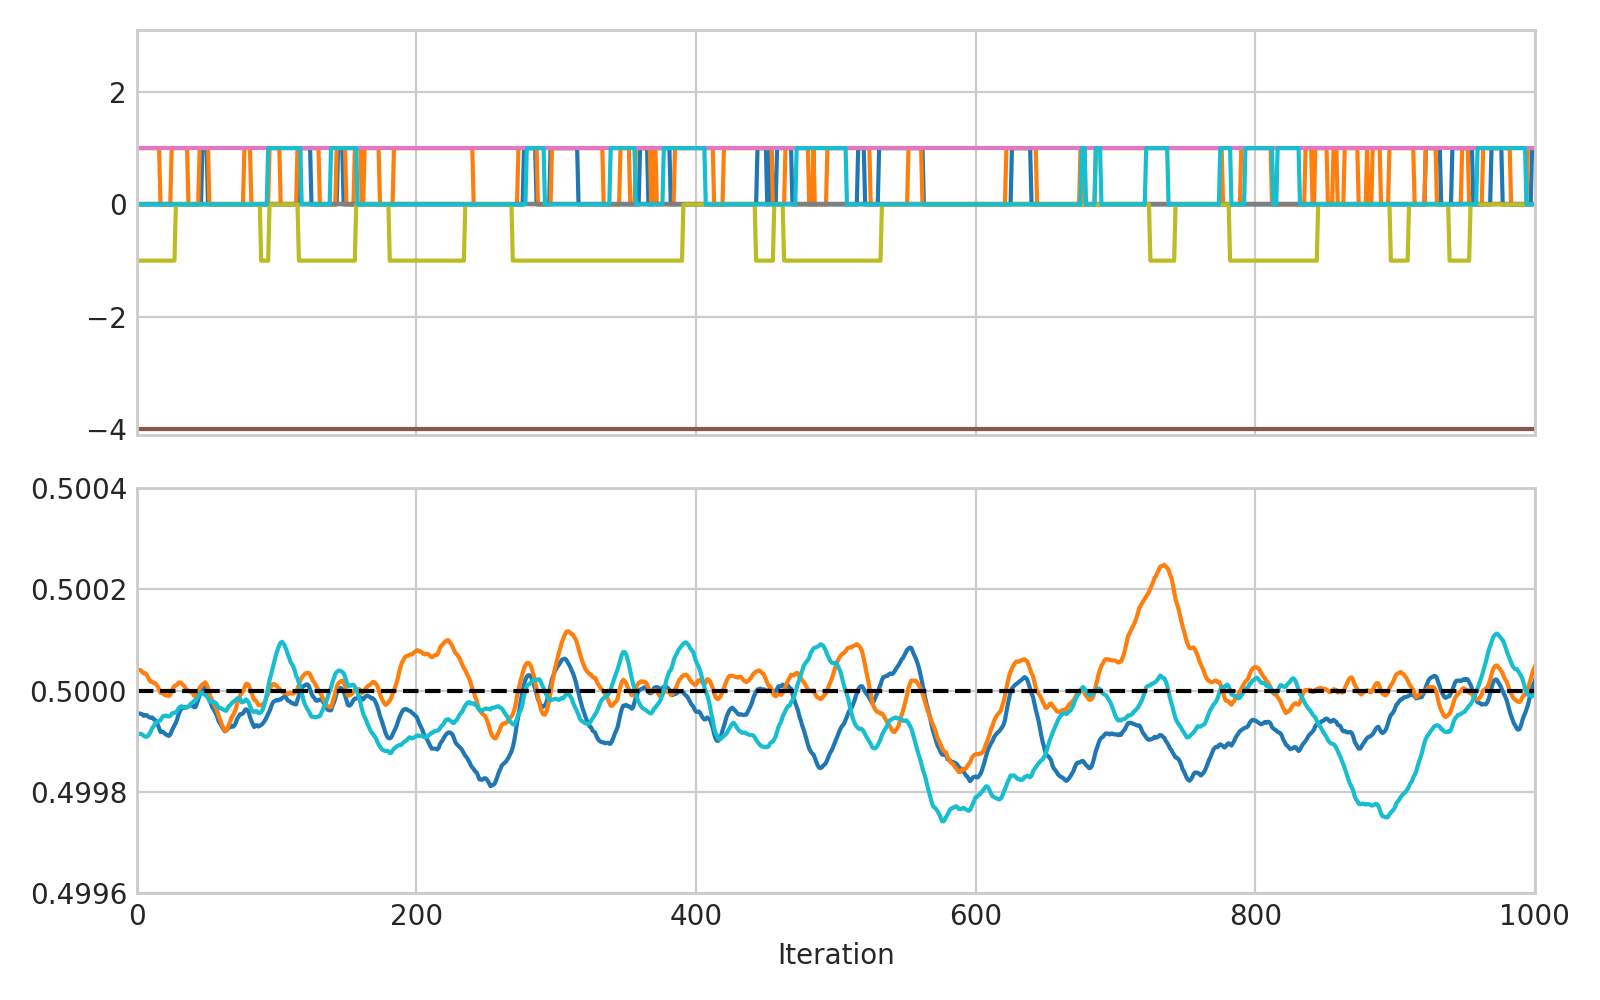
\includegraphics[width=\linewidth]{figures/mnv2_training_oscillation.png} \vspace{-.7cm}
\caption{Progression of weights in the first channel of the first depth-wise separable layer (conv.1.0) during the last 1000 iterations of training \mnv{2} on ImageNet. The top plot shows the integer weights and the bottom plot zooms in on the decision boundary between 0 and 1 for the corresponding latent weights.}
\vspace{-.2cm}
\label{fig:mv2_oscillating_weigths}
\end{figure}

\begin{figure}[t]
\centering
\vspace{-.2cm}
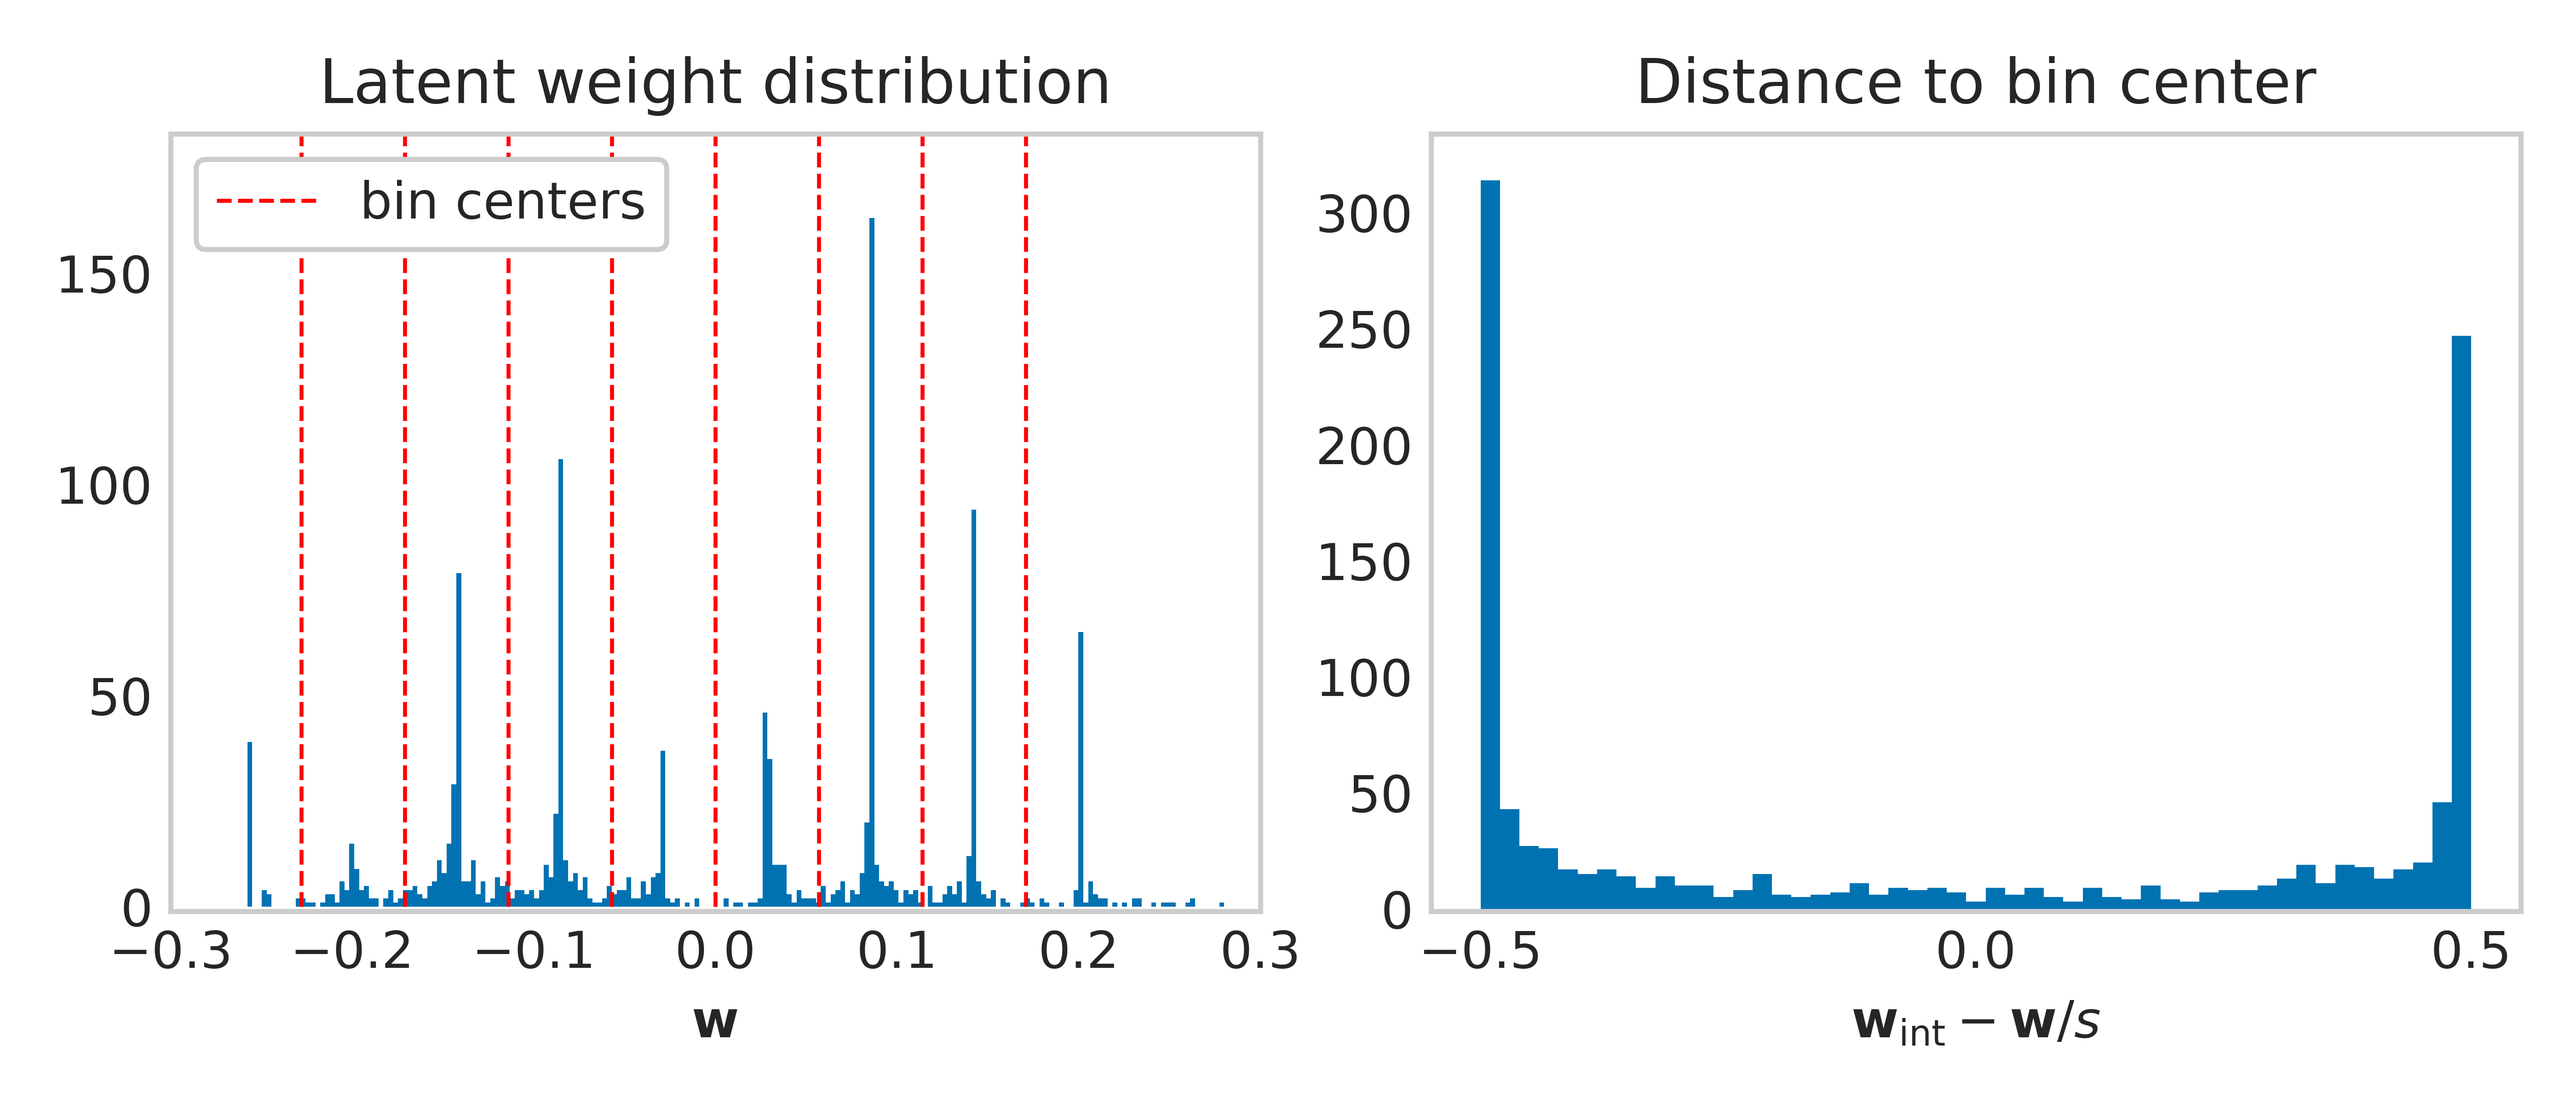
\includegraphics[width=\linewidth]{figures/mnv2_w3_baseline_weigth_dist.png} 
\vspace{-.8cm}
\caption{Weight distribution in depth-wise separable layer of third inverted residual block of \mnv{2} (conv.3.1). Histogram of latent weights (left). Histogram of the distance of latent weight from their closest quantization grid-point ($\vec{w}_{\INT} - \vec{w}/\ct{s}$) (right). 
% We clearly see two peaks close to -0.5 and 0.5 which represent the number of weights close to the decision boundary.
}
\vspace{-.1cm}
\label{fig:mv2_bin_distribution}
\end{figure}

\subsection{Oscillations in practice}
\label{sec:oscillation_in_practice}
These oscillations are not just an unfortunate side-effect of this fictitious toy example. They are indeed present in larger neural networks with significant implications for their optimization. Figure \ref{fig:mv2_oscillating_weigths} shows the progression of 3-bit quantized weights in a depth-wise separable layer of \mnv{2} close to convergence, trained using LSQ \citep{lsq} on ImageNet. We observe that many of the weights appear to randomly oscillate between two adjacent quantization levels. In figure \ref{fig:mv2_bin_distribution}, we also see that after the supposed convergence of the network, a large fraction of the latent weights lie right at the decision boundary between grid points. This further reinforces the observation that a significant proportion of weights oscillate and do not converge. 

We identify two major issues associated with the oscillations in neural network training: Wrong estimation of the batch-normalization \citep{batchnorm} inference statistics, and an adverse effect on the optimization of the network.



\subsubsection{The effect on Batch-Normalization}
\label{sec:effect_on_bn_statistics}
% \paragraph{Option 1} When training full-precision neural networks we can expect that weights will change very slowly close to convergence. As a result, the output statistics of each layer are expected to be quite stable across iterations. However, oscillation can lead to rapid changes of the integer weights during QAT (see in figure \ref{fig:mv2_oscillating_weigths}) leading to significant distribution shift between gradient updates, even close to convergence. Batch-normalization layers track the exponential moving average (EMA) of the mean and variance for each layer's output, so that it can be used during inference as an approximation of the real sample statistics.  The sudden and large changes in output distribution induced by oscillations can corrupt these moving statistics estimates leading to a significant degradation in accuracy. In fact, there are two factors that amplify this effect: the weight bit-width and the number of weights per output channel.


% \paragraph{Option 2} 
% Oscillations in QAT can cause integer weights to change quite rapidly during training (see figure \ref{fig:mv2_oscillating_weigths}) leading to significant distribution shift between gradient updates, even close to supposed convergence. Batch-normalization layers track the exponential moving average (EMA) of the mean and variance for each layer's output, so that it can be used during inference as an approximation of the real sample statistics. The sudden and large changes in output distribution induced by oscillations can corrupt these moving statistics estimates leading to a significant degradation in accuracy. In fact, there are two factors that amplify this effect: the weight bit-width and the number of weights per output channel.

During training  batch-normalization layers track the exponential moving average (EMA) of the mean and variance for each layer's output, so that it can be used during inference as an approximation of the real sample statistics. 
When training full-precision neural networks we can expect that weights will change very slowly close to convergence. As a result, the output statistics of each layer are expected to be quite stable across iterations and therefore the EMA is a good estimate of the statistics.
However, oscillations in QAT can lead to rapid changes of the integer weights (see in figure \ref{fig:mv2_oscillating_weigths}) leading to significant distribution shift between iterations, even close to convergence.
The sudden and large changes in the output distribution induced by oscillations can corrupt the EMA statistics leading to a significant degradation in accuracy. In fact, there are two factors that amplify this effect: the weight bit-width and the number of weights per output channel.
% The fact that many weights oscillate between quantized states, even at the supposed convergence of the network, means that the output statistics of each layer can vary significantly between gradient updates. Batch-normalization layers track the running mean and variance for each layer's output, so that it can be used during inference for any batch-size. These running estimates can be corrupted due to the distribution shift induced by oscillations, leading to a significant degradation in accuracy. In fact, two factors influence this effect: the weight bit-width and the number of weights per output channel.

The lower the bit-width $b$, the larger the distance becomes between quantization levels, as it is proportional to $1/2^b$. As the oscillating weights move from one quantization level to the other, they cause a proportionally larger shift in the output distribution. The second important factor is the number of weights per output channel. The smaller the number of weights, the larger the contribution of individual weights to the final accumulation. When the number of accumulations increases, the effects of oscillations average out due to the law of large numbers. 

In table \ref{tbl:bn_stats_diff}, we use the KL-divergence\footnote{We we assume that population $p$ and estimated $q$ outputs are normally distributed, such that $D_\text{KL}(p,q)=\log{\frac{\sigma^2_2}{\sigma^2_1} + \frac{\sigma^2_1+(\mu_1-\mu_2)^2}{2\sigma_2^2} -\frac{1}{2}}$, where $p(x)=\mathcal{N}(\mu_1, \sigma_1)$ and $q(x)=\mathcal{N}(\mu_2, \sigma_2)$.} to quantify the discrepancy between population and estimated statistics. We indeed observe that KL divergence is much larger for depth-wise separable layers than in point-wise convolutions in \mnv{2} and the full convolutions in \rn{18}.
 
\begin{table}[t]
    \centering
    \begin{tabular}{ l | l | r r}
    \toprule
        % Network   &   Layer &   $\max_i{D^{(i)}_{\text{KL}}}$& $
        % \eopX{i}{{D}^{(i)}_{\text{KL}}}$ \\
                Network   &   Layer &   $\max{D_{\text{KL}}}$& $
        \eop{D_{\text{KL}}}$ \\
        \midrule

        \rn{18} & layer1.0.conv1 &  0.0059 &	0.0002 \\
        \rn{18} & layer1.0.conv2 &  0.0130 &	0.0014 \\
        \rn{18} & layer3.0.conv1 &  0.0006 & 0.0001 \\
        \midrule
        
        \mnv{2} & conv3.0 (PW)  &  0.7858 &   0.0292 \\
        \mnv{2} & conv3.1 (DW)  &  55.3782 &	1.25464 \\
        \mnv{2} & conv3.2 (PW) &  0.0065 &	0.0012 \\
        % \mnv{2} & PWConv3.0  &  0.7858 &   0.0292 \\
        % \mnv{2} & DWConv3.1  &  55.3782 &	1.25464 \\
        % \mnv{2} & PSConv3.2  &  0.00651 &	0.00121 \\
        \midrule
        \mnv{2} & conv10.0 (PW) &  0.0037	& 0.0004 \\
        \mnv{2} & conv10.1 (DW) &  27.2618 & 0.2900\\
        \mnv{2} & conv10.2 (PW)  &  0.0267 &	0.0034\\
        % \mnv{2} & DSConv4  &  0.7858 &   0.0292 \\
        % \mnv{2} & PWConv4  &  0.0024 &   0.0005\\
        % \mnv{2} & DSConv10 &  2.4497 &   0.0626 \\
        % \mnv{2} & PWConv10 &  0.0059 &  0.0010 \\
\bottomrule
\end{tabular}
 \caption{Discrepancy between estimated and actual population statistics of batch-normalization following convolutional layers in \rn{18} and \mnv{2} with weights quantized to 3 bits. We report the maximum and mean KL-divergence across the output channels of each layer. DS: depth-wise separable, PW: point-wise.}\vspace{-.1cm}
 \label{tbl:bn_stats_diff}
\end{table}


A cheap and straightforward solution to this problem is to re-estimate the batch-normalization statistics with a small subset of data after training. This method, which we call \textit{batch-normalization (BN) re-estimation}, is sometimes used in stochastic quantization formulations \citep{peters2018probabilistic,louizos2018relaxed}. However, we argue that it is also essential in deterministic QAT formulations due to the oscillating weights. 

In table \ref{tbl:bn_reestimation_diff}, we see that BN re-estimation not only improves the final quantized accuracy for \mnv{2} but also reduces the variance among different seeds. We further observe that the gap in accuracy widens as the bit-width goes down for \mnv{2}, which is not the case for \rn{18}. 

% It is worth noting that for 8-bits the effect of BN re-estimation is negligible suggesting that this an issue of low-bit quantization. 

%  we observe that gap widens as we reduce the bitwidth, wich confirms the role of the bitwidth .  

% As expected for 

% As expected, the improvement is larger at lower bitwidths and for \mnv{2} with large proportion of depth-wise convolutions compared to \rn{18}, with conventional convolutions. We note that \citet{profit} also observe that low-bit quantization of MobileNets leads to \textit{activation instablity} but fail to recognize the STE-induced oscillations as its source.


\begin{table}[t]
    \centering
    \begin{tabular}{ l | c | c c }
    \toprule
  Network & Bits &  pre-BN & post-BN \\
        \midrule
\rn{18} & 4 & 70.15\textsuperscript{0.03} & 70.20\textsuperscript{0.02} \\
\rn{18} & 3 & 69.63\textsuperscript{0.01}  & 69.70\textsuperscript{0.05} \\
\midrule
\mnv{2}& 8 & 71.79\textsuperscript{0.07}  & 71.89\textsuperscript{0.05}\\ 
\mnv{2}& 4 & 68.99\textsuperscript{0.44} & 71.01\textsuperscript{0.05}\\ 
\mnv{2}& 3 & 64.97\textsuperscript{1.23} & 69.50\textsuperscript{0.04}\\
 % Single run results, run over 3 seeds
\bottomrule
\end{tabular}
 \caption{Validation accuracy (\%) on ImageNet before (pre-BN) and after BN re-estimation (post-BN) for networks trained using low bit weight quantization \citep{lsq} for 20 epochs. We report the average of 3 seeds and the STD in the superscript.}
 \label{tbl:bn_reestimation_diff}
\end{table}

% This effect also happens with other commonly used normalization methods such as Layer-Norm \citep{layernorm}. 

% \todo{Say that this is a low bit issue (as jumps in int get higher), and also stronger in DW separable layers (little weights). Reference PROFIT paper, they say that BN stats}

\begin{table}[t]
    \centering
    \begin{tabular}{ l | c  c }
    \toprule
  Method & Train Loss & Val. Acc. (\%) \\
        \midrule
Baseline         & 1.3566  & 69.50 \\
\midrule
SR (mean + std)  & 1.3547\textsuperscript{0.0053}  & 69.58\textsuperscript{0.09} \\
SR (best)        & 1.3391  & 69.85 \\
AdaRound  & 1.3070  & 70.12 \\
\midrule
Freezing & -  & 70.33 \\
\bottomrule
\end{tabular}
 \caption{Ablation study on the effect of oscillations on QAT. Training loss and validation accuracy (\%) for \mnv{2} with 3-bit weight quantization. SR is stochastic rounding of oscillating weights and AdaRound the binary optimization of oscillating weights.}
\vspace{-.1cm}
 \label{tbl:binary_post_opt}
\end{table}
\subsubsection{The effect on training}
Next to harming the BN statistics, oscillations can also have a negative effect on the training process itself. 
To illustrate this we first show that a converged \mnv{2} with 3-bit weights can achieve a lower training loss (and higher validation accuracy) if we randomly sample oscillating weights between their two oscillating states.
To this end, we sample all weights that were oscillating at the end of training with a probability proportional to the time spent at each quantized state, i.e. $p(\up{w}) = \eopX{t}{w^t = \up{w}}$. We calculate the expectation using a exponential moving average over the integer weights as done in line 15 of algorithm \ref{alg:qat_freezing}.

In table \ref{tbl:binary_post_opt}, we present the results of this experiment. 
% We observe that the mean over the drawn network samples exhibits a loss similar to that of the final converged model. 
We observe that the mean training loss over the sampled networks is similar to that of the final converged model.
However, many samples achieve a lower training loss and the best randomly sampled network shows a significantly lower training loss. 
We also perform a binary optimization of the oscillating weights using an adaptation of AdaRound \citep{adaround}. We optimize the rounding of all layers simultaneously on the final task loss, akin to what is done in the literature with simulated annealing to solve binary optimization problems \citep{Kirkpatrick1983SimulatedAnnealing}. We see that this binary optimization significantly improves over the best stochastic sample and the original converged network. This suggests that weight oscillations prevent the network from converging to the best local minimum during training, and can be detrimental to the optimization process. 

Finally, we show that preventing oscillations earlier in training using our oscillation freezing technique (cf. section \ref{sec:freezing_method}) leads to an even higher validation accuracy than the binary optimization of the oscillating weights. This indicates that the oscillations not only prevent QAT from converging to the best local minimum at the end of training, but can also lead the optimizer towards sub-optimal directions earlier in training. 
% also harm it in finding a better global minimum earlier during training.


% Arguments
% * SGD fails to converge to the best local minima (SR is better than this)
% * Local optimization is worse than intervention 

% Prevents finding good local minima -> better results with bin regularization (both toy example [MF] and MNv2)
% * Question: is it capacity or other optimization issue.

% Setup:
% * Use EMA weights
% * All weigths are rounded
% * For val score, with BN reestimation


% AdaRound:
% * training loss, AdaRound regularization
% * real targets, whole training set
% * BS=64, 10k iters 

